\subsection{Iterator Pattern}

The iterator design pattern aims to simplify the implementation of loops in code
by creating a separate object for traversal. The authors of \cite{GangOf4}
describe: 

\begin{quote}
``The Iterator Pattern provides a way to access the elements of an aggregate 
object without exposing its underlying representation.'' \cite{GangOf4}
\end{quote}

The iterator pattern has many practical use cases including iterating over
groups of collections (often used in conjunction with the Composite design
pattern \cite{GangOf4}), swapping implementations of a given collection (e.g.
from array, to linked list, to vector), optimizing performance (e.g. for a tree
iterator that switches between breadth-first/depth-first strategies), and
filtering results from the iteration.

\begin{figure}[t]
  \begin{center}
  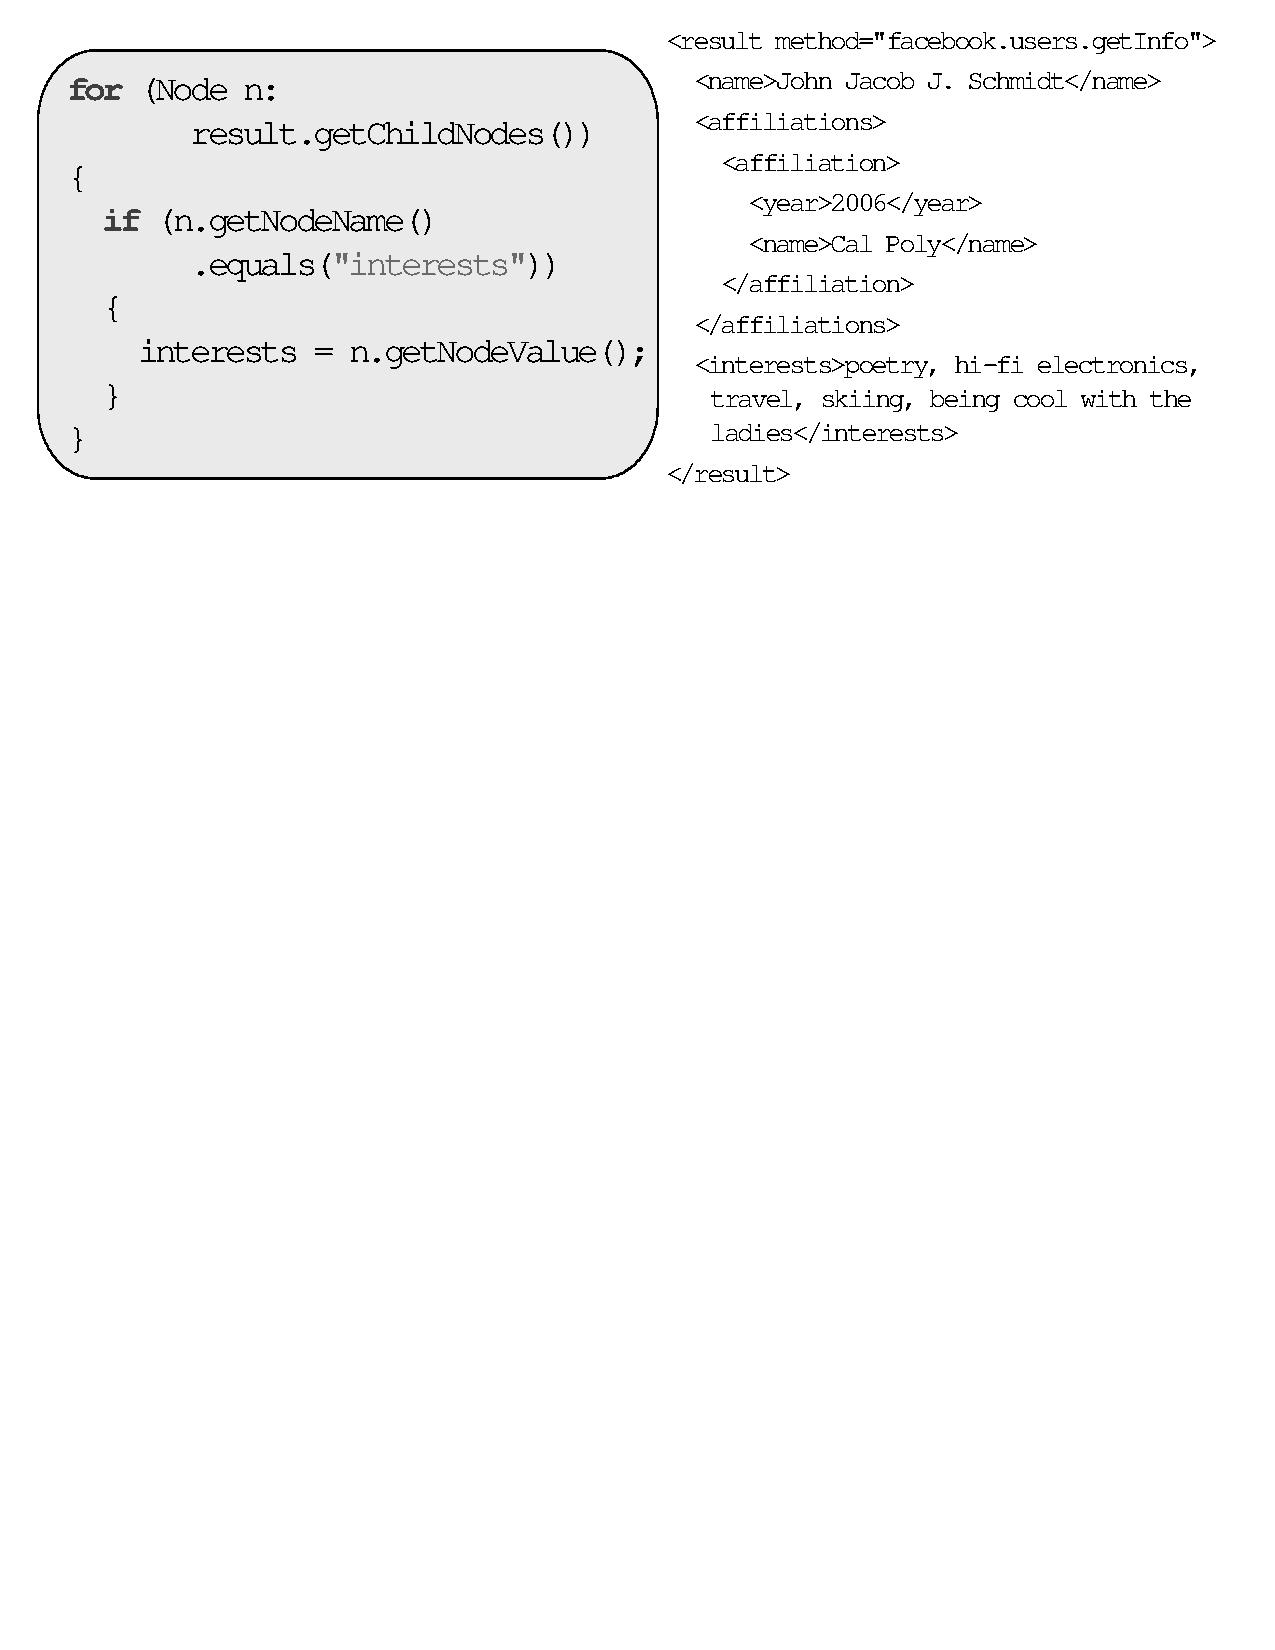
\includegraphics[width=\textwidth]{images/iterator}
  \caption{Iterator Code Samples in Coursebook}
  \label{fig:iterator}
  \end{center}
\end{figure}

In Coursebook, the iterator design pattern is used anywhere that collections are
used. Figure \ref{fig:iterator} shows how the iterator is used to gather data
from the XML return of Facebook web service requests. In the Java code,
\verb!result! is an XML Document instance that has several nodes that contain
data about a user (an XML data sample is shown on the right). When we invoke
\verb!getChildNodes()!, the method returns a collection of XML nodes. This
collection is iterable.

Iterators have become so fundamental to object-oriented programming that since 
the 5.0 Release of the Java Platform, the language now supports enhanced looping
constructs that exploit iterable collections \cite{JSR201}. The Java code in
Figure \ref{fig:iterator} shows this iteration code in use within the Coursebook
web application. When Facebook returns a \verb!NodeList!, we use the enhanced
for loop to find data within the collection.

The iterator is appropriate for several reasons. First, there is an arbitrary
amount of nodes in this collection, so writing a count controlled loop may be
inefficient depending on the implementation of the collection. Second, the XML
data structures used to store the collection of nodes is hidden. Implementors of
the API could decide to change the structure of the collection from tree, to
linked list, to array, and back again. This would not affect our code as long as
the collection remained iterable.
